% This file was created by tikzplotlib v0.9.1.
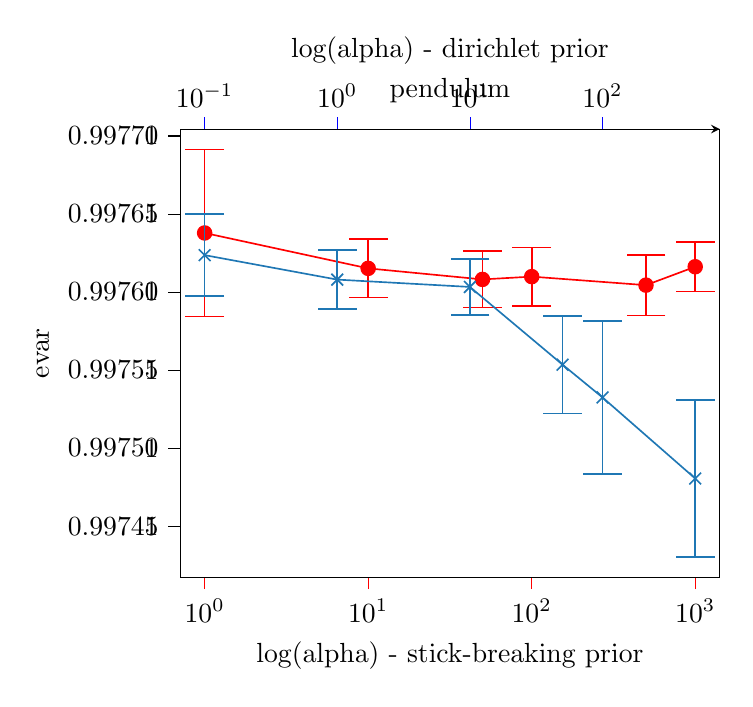
\begin{tikzpicture}

\definecolor{color0}{rgb}{0.12156862745098,0.466666666666667,0.705882352941177}

\begin{axis}[
log basis x={10},
tick align=outside,
tick pos=left,
title={pendulum},
x grid style={white!69.0196078431373!black},
xlabel={log(alpha) - stick-breaking prior},
xmin=0.707945784384138, xmax=1412.53754462275,
xmode=log,
xtick style={color=red},
xtick={0.01,0.1,1,10,100,1000,10000,100000},
xticklabels={\(\displaystyle {10^{-2}}\),\(\displaystyle {10^{-1}}\),\(\displaystyle {10^{0}}\),\(\displaystyle {10^{1}}\),\(\displaystyle {10^{2}}\),\(\displaystyle {10^{3}}\),\(\displaystyle {10^{4}}\),\(\displaystyle {10^{5}}\)},
y grid style={white!69.0196078431373!black},
ylabel={evar},
ymin=0.9974172150527, ymax=0.997704234457134,
ytick style={color=black},
ytick={0.9974,0.99745,0.9975,0.99755,0.9976,0.99765,0.9977,0.99775},
yticklabels={0.99740,0.99745,0.99750,0.99755,0.99760,0.99765,0.99770,0.99775}
]
\path [draw=red, semithick]
(axis cs:1,0.997584246083321)
--(axis cs:1,0.997691188120569);

\path [draw=red, semithick]
(axis cs:10,0.997596368766721)
--(axis cs:10,0.997633732073859);

\path [draw=red, semithick]
(axis cs:50,0.997589978466248)
--(axis cs:50,0.99762598003032);

\path [draw=red, semithick]
(axis cs:100,0.997591146929139)
--(axis cs:100,0.997628386423699);

\path [draw=red, semithick]
(axis cs:500,0.997584866528061)
--(axis cs:500,0.997623742965338);

\path [draw=red, semithick]
(axis cs:1000,0.997600259864805)
--(axis cs:1000,0.997631928992953);

\addplot [semithick, red, mark=-, mark size=7, mark options={solid}, only marks]
table {%
1 0.997584246083321
10 0.997596368766721
50 0.997589978466248
100 0.997591146929139
500 0.997584866528061
1000 0.997600259864805
};
\addplot [semithick, red, mark=-, mark size=7, mark options={solid}, only marks]
table {%
1 0.997691188120569
10 0.997633732073859
50 0.99762598003032
100 0.997628386423699
500 0.997623742965338
1000 0.997631928992953
};
\addplot [semithick, red, mark=*, mark size=2.5, mark options={solid}]
table {%
1 0.997637717101945
10 0.99761505042029
50 0.997607979248284
100 0.997609766676419
500 0.9976043047467
1000 0.997616094428879
};
\end{axis}

\begin{axis}[
axis x line=top,
log basis x={10},
tick align=outside,
x grid style={white!69.0196078431373!black},
xlabel={log(alpha) - dirichlet prior},
xmin=0.0653208007180445, xmax=765.452956031933,
xmode=log,
xtick pos=right,
xtick style={color=blue},
xtick={0.001,0.01,0.1,1,10,100,1000,10000},
xticklabels={\(\displaystyle {10^{-3}}\),\(\displaystyle {10^{-2}}\),\(\displaystyle {10^{-1}}\),\(\displaystyle {10^{0}}\),\(\displaystyle {10^{1}}\),\(\displaystyle {10^{2}}\),\(\displaystyle {10^{3}}\),\(\displaystyle {10^{4}}\)},
y grid style={white!69.0196078431373!black},
ymin=0.9974172150527, ymax=0.997704234457134,
ytick pos=left,
ytick style={color=black}
]
\path [draw=color0, semithick]
(axis cs:0.1,0.997597255345504)
--(axis cs:0.1,0.997649787475757);

\path [draw=color0, semithick]
(axis cs:1,0.997588859207616)
--(axis cs:1,0.997626846755885);

\path [draw=color0, semithick]
(axis cs:10,0.997585127744962)
--(axis cs:10,0.997621200225175);

\path [draw=color0, semithick]
(axis cs:50,0.997522121883669)
--(axis cs:50,0.997584654274979);

\path [draw=color0, semithick]
(axis cs:100,0.997483312219522)
--(axis cs:100,0.997581518633193);

\path [draw=color0, semithick]
(axis cs:500,0.997430261389265)
--(axis cs:500,0.997530757458324);

\addplot [semithick, color0, mark=-, mark size=7, mark options={solid}, only marks]
table {%
0.1 0.997597255345504
1 0.997588859207616
10 0.997585127744962
50 0.997522121883669
100 0.997483312219522
500 0.997430261389265
};
\addplot [semithick, color0, mark=-, mark size=7, mark options={solid}, only marks]
table {%
0.1 0.997649787475757
1 0.997626846755885
10 0.997621200225175
50 0.997584654274979
100 0.997581518633193
500 0.997530757458324
};
\addplot [semithick, color0, mark=x, mark size=3, mark options={solid}]
table {%
0.1 0.99762352141063
1 0.99760785298175
10 0.997603163985069
50 0.997553388079324
100 0.997532415426358
500 0.997480509423795
};
\end{axis}

\end{tikzpicture}
